%%%%%%%%%%%%%%%%%%%%%%%%%%%%%%%%%%%%%%%%%
% NIH Grant Proposal for the Specific Aims and Research Plan Sections
% LaTeX Template
% Version 1.0 (21/10/13)
%
% This template has been downloaded from:
% http://www.LaTeXTemplates.com
%
% Original author:
% Erick Tatro (erickttr@gmail.com) with modifications by:
% Vel (vel@latextemplates.com)
%
% Adapted from:
% J. Hrabe (http://www.magalien.com/public/nih_grants_in_latex.html)
%
% License:
% CC BY-NC-SA 3.0 (http://creativecommons.org/licenses/by-nc-sa/3.0/)
%
%%%%%%%%%%%%%%%%%%%%%%%%%%%%%%%%%%%%%%%%%

%----------------------------------------------------------------------------------------
%	PACKAGES AND OTHER DOCUMENT CONFIGURATIONS
%----------------------------------------------------------------------------------------

\documentclass[11pt,notitlepage]{article}

% A note on fonts: As of 2013, NIH allows Georgia, Arial, Helvetica, and Palatino Linotype. LaTeX doesn't have Georgia or Arial built in; you can try to come up with your own solution if you wish to use those fonts. Here, Palatino & Helvetica are available, leave the font you want to use uncommented while commenting out the other one.
%\usepackage{palatino} % Palatino font
\usepackage[utf8x]{inputenc}%codifica
\usepackage{helvet} % Helvetica font
\usepackage{multirow}
\renewcommand*\familydefault{\sfdefault} % Use the sans serif version of the font
\usepackage[T1]{fontenc}
\linespread{1.2} % A little extra line spread is better for the Palatino font
\usepackage{fancyhdr} %pacchetto per le intestazioni
\usepackage{hyperref}
\usepackage{lipsum} % Used for inserting dummy 'Lorem ipsum' text into the template
\usepackage{amsfonts, amsmath, amsthm, amssymb} % For math fonts, symbols and environments
\usepackage{graphicx} % Required for including images
%\usepackage{booktabs} % Top and bottom rules for table
%\usepackage{wrapfig} % Allows in-line images
%\usepackage[labelfont=bf]{caption} % Make figure numbering in captions bold
\usepackage[top=0.5in,bottom=0.5in,left=0.5in,right=0.5in]{geometry} % Reduce the size of the margin
\usepackage{pdflscape}
\pagestyle{empty}

\hyphenation{ionto-pho-re-tic iso-tro-pic fortran} % Specifies custom hyphenation points for words or words that shouldn't be hyphenated at all

\hypersetup{
	colorlinks=true,
	linkcolor=black,
	urlcolor=blue
}

%----------------------------------------------------------------------------------------
%	Creato da Mich
%----------------------------------------------------------------------------------------

\begin{document}
	
\noindent
\parbox{0.7\columnwidth}{Università degli Studi di Padova\\
	Piano di lavoro stage presso Mivoq S.r.l.\\
	Matteo Lisotto (1052736)}%matricola
\parbox{0.3\columnwidth}{
	\hfill 
\includegraphics[scale=0.08]{immagini/logo-unipd.png}}

\bigskip
\begin{center}
{\Huge \textbf{Piano di lavoro}} \\ \bigskip
	{\Large \textit{presso Mivoq S.r.l.}}\\ \bigskip
	{\Large \textit{Matteo Lisotto}}
\end{center}

\section*{Contatti}
\textbf{Studente:} Matteo Lisotto, \href{mailto:matteo.lisotto@studenti.unipd.com}{matteo.lisotto@studenti.unipd.com}, 3336492471 \\
\textbf{Tutor aziendale:} Giulio Paci, \href{mailto:giulio.paci@mivoq.it}{giulio.paci@mivoq.it}, 049 0998335 \\
\textbf{Azienda:} Mivoq S.r.l., via Martiri della libertà 2, 35137 Padova (PD), \href{www.mivoq.it}{www.mivoq.it}

\section*{Scopo dello stage}

L'azienda si occupa di sviluppare prodotti software riguardanti la sintesi vocale.\\

\noindent Lo stage prevede l'inserimento dello studente nel team di ricerca e sviluppo. Lo studente verrà formato nel campo della sintesi vocale e dell'analisi del linguaggio naturale in particolare.\\ 

\noindent I principali argomenti trattati saranno:
\begin{itemize}
	\item componenti base per l'analisi del testo in un sistema di sintesi vocale;
	\item machine learning applicato all'analisi del linguaggio naturale;
	\item valutazione di sistemi di analisi del linguaggio naturale.
\end{itemize}

\newpage

\noindent
\parbox{0.7\columnwidth}{Università degli Studi di Padova\\
	Piano di lavoro stage presso Mivoq S.r.l.\\
	Matteo Lisotto (1052736)}
\parbox{0.3\columnwidth}{
	\hfill 
\includegraphics[scale=0.08]{immagini/logo-unipd.png}}

\bigskip
\section*{Pianificazione del lavoro}
La pianificazione, in termini di quantità di ore di lavoro, sarà così distribuita:

\begin{center}
	
\begin{tabular}{|l|l|c l|}
	\hline
	\multicolumn{2}{|l|}{\textbf{Durata in ore}}		&	\multicolumn{2}{l|}{\textbf{Descrizione dell'attività}}\\
	\hline
	\multicolumn{2}{|l|}{72}	&	\multicolumn{2}{l|}{Setup di speect e analisi del codice}\\
	\hline
	\multirow{3}{1cm}{ }    &            16            &            \hspace{5mm}•\hspace{2mm}            & Setup del sistema e di una voce di esempio inglese \\
	\cline{2-2}
	&            56            &            \hspace{5mm}•\hspace{2mm}            &            Analisi del codice e delle funzioni principali\\
	\hline
	
	\multicolumn{2}{|l|}{248}	&	\multicolumn{2}{l|}{Implementazione di un frontend linguistico per l'Italiano}\\
	\hline

	\multirow{3}{1cm}{ }    &            40            &            \hspace{5mm}•\hspace{2mm}            & Implementazione di un tokenizer basato su regole \\
	\cline{2-2}
	&            80            &            \hspace{5mm}•\hspace{2mm}            &            Implementazione di un POS tagger basato su esempi \\
	\cline{2-2}
	&            80            &            \hspace{5mm}•\hspace{2mm}            &            Implementazione di un trascrittore fonetico \\
	\cline{2-2}
	&            48            &            \hspace{5mm}•\hspace{2mm}            &            Valutazione delle componenti del frontend e confronto con MaryTTS  \\
	\hline
\end{tabular}

\end{center}

\section*{Obiettivi}

Si farà riferimento ai requisiti secondo le seguenti notazioni:
\begin{itemize}
	\item «ob» per i requisiti obbligatori, vincolanti in quanto obiettivo primario
	richiesto dal committente;
	\item  «de» per i requisiti desiderabili, non vincolanti o strettamente necessari,
	ma dal riconoscibile valore aggiunto;
	\item «op» per i requisiti opzionali, rappresentanti valore aggiunto non
	strettamente competitivo.
\end{itemize}
Le sigle precedentemente indicate saranno seguite da una coppia sequenziale di numeri, identificativo del requisito.\\

\newpage

\noindent
\parbox{0.7\columnwidth}{Università degli Studi di Padova\\
	Piano di lavoro stage presso Mivoq S.r.l.\\
        Matteo Lisotto (1052736)}
\parbox{0.3\columnwidth}{
	\hfill 
\includegraphics[scale=0.08]{immagini/logo-unipd.png}}

\bigskip
\bigskip
\noindent
Si prevede lo svolgimento dei seguenti obiettivi:
\begin{itemize}
	\item Obbligatori
	\begin{itemize}
		\item \underline{\textit{ob01}}: Implementazione di un tokenizer per l'Italiano;
		\item \underline{\textit{ob02}}: Implementazione di un POS tagger per l'Italiano;
		\item \underline{\textit{ob03}}: Implementazione phonemizer per l'Italiano;
		\item \underline{\textit{ob03}}: Valutazione dei risultati del tokenizer;
		\item \underline{\textit{ob04}}: Valutazione dei risultati del POS tagger;
		\item \underline{\textit{ob05}}: Valutazione dei risultati del phonemiser;
	\end{itemize}
	
	\item Desiderabili 
	\begin{itemize}
                \item \underline{\textit{de01}}: Implementazione di regole di espansione nel tokenizer;
                \item \underline{\textit{de02}}: Implementazione di un sistema di disambiguazione per il phonemiser;
                \item \underline{\textit{de03}}: Automatizzazione della valutazione dei risultati del tokenizer;
		\item \underline{\textit{de04}}: Automatizzazione della valutazione dei risultati del POS tagger;
		\item \underline{\textit{de05}}: Automatizzazione della valutazione dei risultati del phonemiser;
	\end{itemize}
\end{itemize}


\section*{Diagramma di Gantt}
Di seguito è riportato il diagramma di Gantt relativo al piano di lavoro previsto.
\newpage

\begin{landscape}
\begin{center}
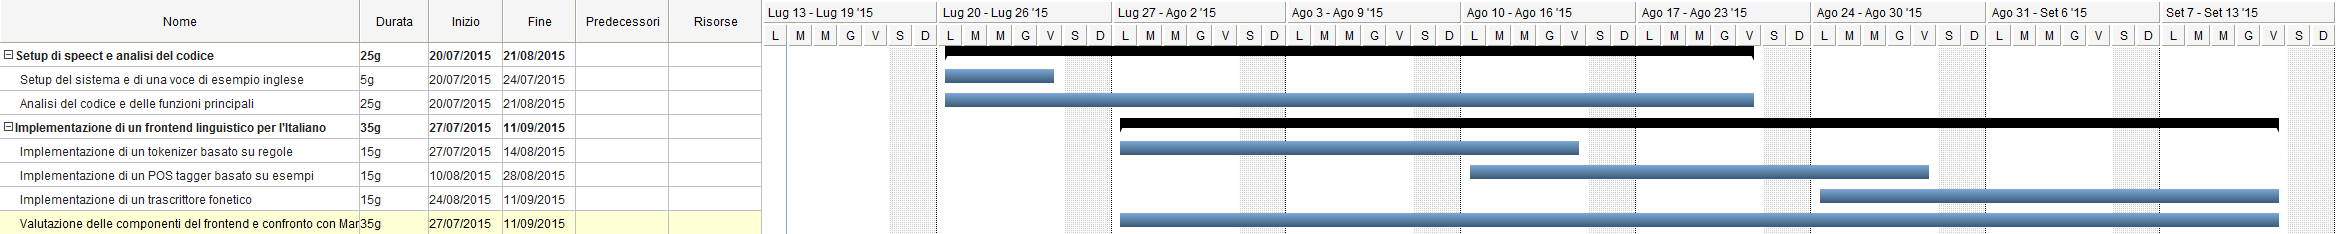
\includegraphics[scale=0.40]{immagini/gantt.png}
\end{center}
\end{landscape}
\end{document}
